% !TEX encoding = UTF-8 Unicode

\chapter{Tworzenie zbiorów danych}
Priorytetem było stworzenie zestawu danych
umożliwiającego rozwój różnych modeli sieci neuronowych bez konieczności każdorazowego
ingerowania w zbiór lub dopasowywania go specjalnie do konkretnej sieci.\\
\textbf{Wszystkie zbiory dostępne są pod linkami w części Dodatek A [\ref{dodatekA}] }

\section{Uzyskiwanie zbiorów ze zdjeć}
Ilość zdjęć wykonanych ręcznie z wykorzystaniem kamery była zbyt mała by sieć bezpośrednio
z nich korzystała. Oprócz tego rozmiar zdjęć 1600x1200 był na tyle duży, że bardzo wydlużyłby
proces uczenia sieci.\\
Rozwiązaniem obu problemów było zwiększenie ilości zdjęć przy jednoczesnym zmniejszeniu
ich rozmiarów. Do wszystkich obrazów wykorzystywanych w tej pracy, zastosowano następujące
kroki:
\begin{itemize}
\item Skalowanie obrazów
\item Przekształcanie \textit{(ang. warping)} na kilka różnych sposobów by uzyskać lekko zdeformowane kostki
\item Rotacja o określony kąt by umożliwić rozpoznawanie kości niezależnie od jej obrotu
\item Kadrowanie obrazu do pożądanej wielkości
\end{itemize}
Wszystkie zbiory wykorzystane w tej pracy były podzielone na części treningową i testową
w stosunku 4:1, niezależnie od ich liczebności.

\section{Zbiór obrazów kwadratowych}
Pierwszy stworzony zbiór składał się z obrazów kwadratowych. Było to podyktowane
faktem, że praktycznie wszystkie przykłady użycia sieci neuronowych do rozpoznawania
obrazów korzystały z kwadratowych zdjeć.\\
Najważniejszym założeniem przy tworzeniu zbioru było uzyskanie zdjęć kości położonej
na środku obrazu z kamery, na obszarze kwadratu o boku długości około 3 krotnie większej
niż długość ściany samej kości. Pozwalało to uzyskać niewielkie rozmiary obrazów 64x64 piksele,
gdzie kość stanowiła około 14\%, a jedno oczko 0,2\% powierzchnii.\\
Kolejną kwestią było przystosowanie sieci do rozpoznawania kości o różnych kolorach ścian,
oczek i samego tła. W związku z tym zdjęcia podzielono na zestawy, z których każdy miał ustaloną
barwę tła, kości oraz oczek. Każda ścianka sfotografowana była od 3 do 30 razy, dająć
liczebność każdego z zestaów miedzy 18 a 180 zdjęć. Niektóre zdjęcia poddawane były
działaniu ostrego, punktowego światła w celu wygenerowania trudniejszych do rozpoznania obrazów.
Zestawienia kolorystyczne wypisane są w tabeli poniżej \ref{tab:zestawienie1}.

\begin{table}[h!]
\centering
\begin{tabular}{rcl|cc}
\multicolumn{3}{c}{Kolor} & \multicolumn{2}{c}{Ilość zdjęć} \\ \hline
kości & oczek & tła & ściany & kostki \\ \hline
biały & czarny & czerwony & 30 & 180 \\
biały & czarny & granatowy & 3 & 18 \\
biały & czarny & czarny & 8 & 48 \\
beżowy & czarny & czerwony & 3 & 18 \\
czarny & biały & czarny & 10 & 60 \\
czarny & biały & czerwony & 10 & 60 \\
czerwony & biały & czerwony & 5 & 30 \\
czerwony & czarny & czerwony & 3 & 18 \\
granatowy & złoty & biały & 4 & 24 \\
granatowy & złoty & niebieski & 6 & 36 \\
zielony & biały & zielony & 8 & 48 \\
zielony & biały & biały & 5 & 30 \\
różowoczerwony & czarny & biały & 5 & 30 \\ \hline
\multicolumn{3}{c}{\textit{Łączna ilość zdjęć:}} & \textit{100} & \textit{600}
\end{tabular}
\vspace{0.2cm}
\caption{Zestawienie kolorystyczne obrazów 1}
\label{tab:zestawienie1}
\end{table}
Po wykonaniu zdjęć każde z nich zostało poddane obróbce w celu zmniejszenia i uzyskania licznych,
zróżnicowanych zbiorów. W przypadku zbioru kwadratowego wszystkie zdjęcia zostały przeskalowane
do 18,66\% początkowego rozmiaru (stosunek 5,36:1). Następnie poddano je 6 przekształceniom, które
rozciągały lub zwężały obrazy o 1-5\% z różnych strony. Kolejnym krokiem był obrót o kąt
15\textsuperscript{o} lub 30\textsuperscript{o}, zależnie czy dany zbiór wykorzystywany był w mniej
lub bardziej rozbudowanych sieciach. Ostatnią operacją było kadrowanie zdjęć do rozmairu 64x64 piksele.\\
Powyższe działania spowodowały uzyskanie 84 lub 168 zdjęć o rozmiarze 64x64 z każdego
z początkowych obrazów o rozmiarze 1600x1200 pikseli. Pełne zbiory liczyły 50400 i 100800
obrazów, jednakowo w wersjach kolorowych RGB oraz w odcieniach skali szarości.
Wybrane zdjęcia ze zbioru znajdują się na rysunku \ref{fig:squares} poniżej: \newpage

\begin{figure}[h!]
\centering
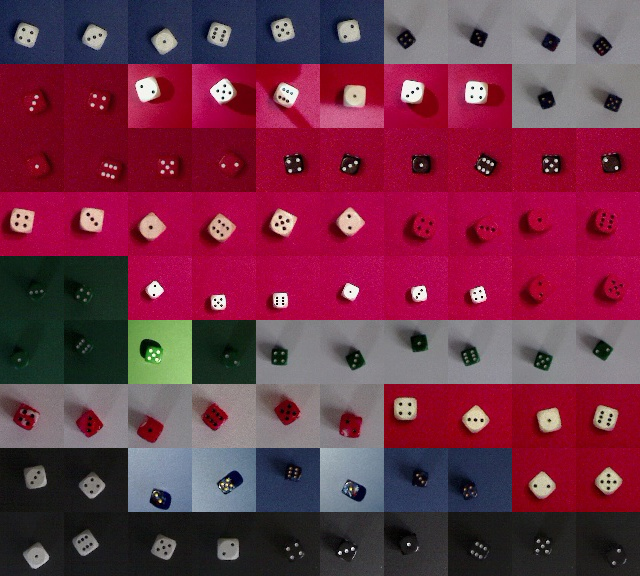
\includegraphics[scale=0.35]{images/kolaz}
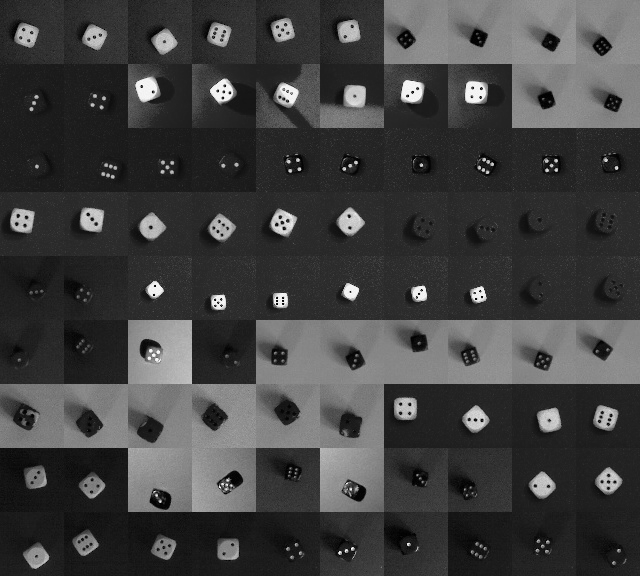
\includegraphics[scale=0.35]{images/kolaz_grayscale}
\caption{Obrazy o rozdzielczościach 64x64}
\label{fig:squares}
\end{figure}

\section{Zbiór obrazów prostokątnych}
Po wytrenowaniu kilku sieci na zbiorach kwadratowych, zdecydowano się na wykorzystanie
większych obrazów, które zachowują kształt prostokątny i stosunek szerokości do wysokości
identyczny jak w obrazie otrzymywanym z kamery. Miało to ułatwić detekcję kości na obrazie,
ponieważ obszar 64x64 pikseli był na tyle niewielki, że ciężko w niego trafić podczas
rzutu kostką.\\
Bardzo istotną rzeczą w tym zbiorze był fakt, że pomimo większego rozmiaru zdjęć, stosunek
rozmiaru kości do całego zdjęcia był zdecydowanie mniejszy. W zdjęciach kwadratowych kostka
zajmowała 14\%, natomiast w prostokątnych jedynie 2\% powierzchnii obrazu, a dodatkowo pojedyncze
oczko to tylko 0,08\% powierzchnii.
Dla zwiększenia trudności kości były rozmieszczane w bardziej zróżnicowany sposób, nie skupiały
się jedynie wokół środka obrazu. Do wykonanych na potrzeby poprzedniego zbioru zdjęć, dodano
nowe i tak utworzono kilkanaście zestawień kolorystycznych, przedstawionych w poniższej tabeli \ref{tab:zestawienie2} \newpage

\begin{table}[h!]
\centering
\begin{tabular}{rcl|cc}
\multicolumn{3}{c}{Kolor} & \multicolumn{2}{c}{Ilość zdjęć} \\ \hline
kości & oczek & tła & ściany & kostki \\ \hline
biały & czarny & czerwony & 30 & 180 \\
biały & czarny & granatowy & 3 & 18 \\
biały & czarny & czarny & 8 & 48 \\
beżowy & czarny & czerwony & 3 & 18 \\
czarny & biały & czarny & 10 & 60 \\
czarny & biały & czerwony & 10 & 60 \\
czerwony & biały & czerwony & 5 & 30 \\
czerwony & czarny & czerwony & 3 & 18 \\
granatowy & złoty & biały & 4 & 24 \\
granatowy & złoty & niebieski & 6 & 36 \\
zielony & biały & zielony & 8 & 48 \\
zielony & biały & biały & 5 & 30 \\
różowoczerwony & czarny & biały & 5 & 30 \\ \hline
biały & czarny & zielony & 6 & 36 \\
czerwony & biały & zielony & 6 & 36 \\
czerwony & czarny & różowy & 7 & 42 \\
czarny & biały & szary & 6 & 36 \\
czarny & biały & niebieski & 6 & 36 \\
beżowy & czarny & szary & 6 & 36 \\
beżowy & czarny & niebieski & 6 & 36 \\
granatowy & złoty & biały & 8 & 48 \\
zielony & biały & żółty & 7 & 42 \\
różowoczerwony & czarny & pomarańczowy & 6 & 36 \\ \hline
\multicolumn{3}{c}{\textit{Łączna ilość zdjęć:}} & \textit{164} & \textit{984}
\end{tabular}
\vspace{0.2cm}
\caption{Zestawienie kolorystyczne obrazów 2}
\label{tab:zestawienie2}
\end{table}
Tak jak poprzednio, zdjęcia zostały poddane obróbce. Początkowo wszystkie zostały
przeskalowane do 0,165\% początkowego rozmiaru (stosunek 6:1). Następnie poddano je 4,
analogicznym jak poprzednio przekształceniom. Dokonano również rotacji o kąt 30\textsuperscript{o}
i skadrowanie zdjęć do rozmairu 106x79 pikseli.\\
Uzyskano w ten sposób 60 zdjęć o rozmiarze 106x79 z każdego poczatkowego zdjęcia.
Obrazy zastosowane w sieciach występowały jedynie w odcieniach skali szarości.
Całkowita ilość obrazów w pełnym zbiorze danych wynosiła 59040, co przełożyło się
na 47232 obrazów treningowych i 11808 testowych. Przykładowe zdjęcia ze zbioru znajdują
się na rysunku \ref{fig:rects} poniżej

\begin{figure}[h!]
\centering
\includegraphics[scale=0.5]{dices_106x79}
\caption{Obrazy o rozdzielczościach 106x79}
\label{fig:rects}
\end{figure}
